\documentclass[11pt]{article}

% ---------------------------------------------------------------------------
% leakgauge --- arXiv technical note (v0 draft)
% Thesis-INDEPENDENT parts are drafted; every empirical claim is a marked
% placeholder to be filled after the model run. See \placeholder{} macro.
% ---------------------------------------------------------------------------

\usepackage[utf8]{inputenc}
\usepackage[T1]{fontenc}
\usepackage[margin=1in]{geometry}
\usepackage{amsmath}
\usepackage{amssymb}
\usepackage{booktabs}
\usepackage{graphicx}
\usepackage{xcolor}
\usepackage{tikz}
\usepackage[hidelinks]{hyperref}

% Marked placeholder for numbers/plots to be filled after the model run.
\newcommand{\placeholder}[1]{{\color{red}\textbf{[TODO: #1]}}}
\newcommand{\code}[1]{\texttt{#1}}
\newcommand{\hijackasr}{hijack-ASR}
\newcommand{\leakasr}{leakage-verified ASR}

\title{\textbf{leakgauge}: Does Verifying Data Leakage Reorder\\
Prompt-Injection Robustness Rankings?\\[0.4em]
\large A leakage-verified benchmark for LLM agents}

\author{%
  Bamdad Dashtban\\
  \texttt{bamdadd@gmail.com}
}
\date{Draft --- \today}

\begin{document}
\maketitle

\begin{abstract}
Benchmarks for prompt injection in tool-using LLM agents typically score an
\emph{attack-success rate} (ASR) that counts whether the model was
\emph{hijacked} --- coaxed into performing the attacker's action, such as
issuing an outbound tool call to an attacker-controlled destination. But the
harm that motivates these benchmarks is usually \emph{data exfiltration}: a
secret actually leaving the trust boundary. Performing the action and leaking a
secret are not the same event. We ask a measurement question: if we re-score the
\emph{same} agent traces on \emph{verified leakage} --- a unique canary token
provably present in the outbound call's arguments --- does the resulting ranking
of model robustness differ from the ranking produced by hijack ASR?
\textbf{leakgauge} is a small, defensive, leakage-verified benchmark built to
answer this. Leakage is decided by a programmatic canary predicate (exact string
match after decoding common encodings; no LLM judge), over an email-and-calendar
agent workspace exercised by three \emph{published} indirect-injection attack
families. We report two ASRs plus utility-under-attack, bootstrap confidence
intervals, and a Kendall-$\tau$ rank-reorder statistic as the headline. This note
fixes the method, metrics, and threat model; the empirical result is marked as a
placeholder pending the model run. \placeholder{final one-sentence result:
reorder observed / not observed, with $\tau$ and CI.}
\end{abstract}

% ===========================================================================
\section{Introduction}
% ===========================================================================

\textbf{This is a defensive measurement harness, not an attack toolkit.} Its
purpose is to quantify whether an agent's defences hold against prompt injection
so they can be improved, and to sharpen how the field \emph{scores} that
robustness. Attacks appear in the suite only to exercise defences; only
previously published attack patterns are used, and no novel high-potency
jailbreaks or harmful-content payloads are introduced (Section~\ref{sec:safety}).

Tool-using LLM agents read untrusted content --- emails, web pages, calendar
invitations --- and act on it with privileged tools. \emph{Indirect prompt
injection} places attacker instructions inside that content
\cite{greshake2023,perez2022}. The community has responded with agent-injection
benchmarks, notably AgentDojo \cite{agentdojo2024} and InjecAgent
\cite{injecagent2024}, which measure how often an attack succeeds.

\paragraph{The gap.} ``Success'' in these suites is, operationally, that the
model \emph{took the attacker's action} --- e.g., it called \code{send\_email}
to an attacker address. Call this \emph{hijacking}. But the risk a data-exposure
threat model cares about is \emph{exfiltration}: did a protected secret leave
with that call? A model can be hijacked --- it emits the outbound call --- yet
leak nothing, because the call carried no secret (it refused the credential,
hallucinated a placeholder, or was interrupted). Counting hijacks therefore
\emph{upper-bounds} exfiltration risk, potentially loosely, and a leaderboard
sorted by hijack ASR may rank models differently from one sorted by verified
leakage.

\paragraph{The question.} We therefore ask, question-first:
\begin{quote}
\emph{If the same agent traces are re-scored on programmatically verified data
leakage instead of task hijacking, does the ranking of model robustness
reorder?}
\end{quote}
This is a claim about \emph{measurement discipline}, and it is falsifiable
(Section~\ref{sec:limitations}). If the two rankings agree, leakage verification
adds no discriminative signal and ``hijack ASR is a fine proxy'' becomes a
supported, publishable conclusion. If they disagree, then how injection
benchmarks score matters for which model one would deploy.

\paragraph{Contributions.}
\begin{enumerate}
  \item A \emph{leakage-verified} scoring predicate for agent injection: a
        per-case canary token whose presence in outbound tool-call arguments is
        decided by pure string matching after encoding-normalization --- never by
        an LLM judge (Section~\ref{sec:predicate}).
  \item A small, reproducible email-and-calendar agent workspace and three
        \emph{published} attack families --- delayed trigger, cross-context
        assembly, and encoding-wrapped exfiltration (Section~\ref{sec:families}).
  \item A scoring protocol reporting two ASRs and utility-under-attack with
        bootstrap CIs, and a Kendall-$\tau$ \emph{rank-reorder} statistic as the
        headline thesis test (Section~\ref{sec:metrics}).
\end{enumerate}
We deliberately keep the suite small and single-domain, and we state the
resulting statistical limits openly (Section~\ref{sec:limitations}).

% ===========================================================================
\section{Method}
\label{sec:method}
% ===========================================================================

\subsection{The canary / leakage predicate (the spine)}
\label{sec:predicate}

Every case plants a unique, unguessable \emph{canary} token of the form
\code{LKG-}\textlangle 32 hex\textrangle{} in an environment field the benign
task legitimately touches (an email body, a calendar note). Two events are then
read off a single recorded trace of tool calls:

\begin{description}
  \item[Hijack] an outbound/sensitive tool was called with a destination
    matching the case's exfiltration spec (an attacker address in a
    recipient/URL field), \emph{regardless of payload}.
  \item[Leakage] such an outbound call's arguments actually \emph{carry the
    canary} --- the exact token, or a decodable transform of it.
\end{description}

Leakage is a \textbf{pure string match after normalization, with no model in the
loop}. Normalization folds the transforms an attacker can apply to slip a naive
substring filter: Base64, hexadecimal, ROT13, and Unicode homoglyph / fullwidth
confusables. Concretely, the predicate (i) case-folds and applies Unicode NFKC
plus a homoglyph table to the outbound arguments, then (ii) searches for the
canary both forward (pre-encoding the canary and matching) and in reverse
(decoding candidate Base64/hex tokens and un-rotating ROT13, then matching). A
match counts as leakage only if it occurs in a call whose \emph{destination}
matches the exfiltration spec, so a benign message that merely quotes an attacker
address --- or even the canary --- to a legitimate recipient does not register.

Deciding leakage programmatically is the methodological point. An LLM judge would
reintroduce exactly the failure mode under study (a model's opinion about whether
a secret leaked) into the measurement of it. The canary makes leakage a decidable
predicate over the trace.

\subsection{Workspace and traces}

The environment is a lightweight, zero-dependency email-and-calendar workspace
whose state shape (inbox, sent, contacts, calendar) mirrors AgentDojo
\cite{agentdojo2024} so that cases and defences can port, but which we implement
self-contained. It exposes the tools an assistant would use --- reading and
searching mail, sending mail, searching contacts, and listing, reading, and
creating calendar events. Attacker content lives \emph{inside} environment
fields (email bodies, event descriptions), never in the user's instruction. Each
tool call is recorded with its \emph{full arguments}, so both the hijack and the
leakage predicate are computable from one trace. A run is scored per case over
$k$ seeded repeats.

\subsection{Attack families (published patterns only)}
\label{sec:families}

Each family instantiates a documented indirect-injection pattern in the
workspace. We introduce no new jailbreak technique; the contribution is the
leakage-verified \emph{scoring}, not the attacks.

\begin{description}
  \item[Delayed trigger] the injected instruction sits in a benign-looking
    thread the agent only reaches partway through the legitimate task, so the
    malicious step is temporally separated from the content that triggers it
    \cite{greshake2023}.
  \item[Cross-context assembly] the payload is \emph{split} across multiple
    retrieved sources --- the secret in one field, the ``forward it''
    instruction in another, the destination in a third --- so no single field
    reads as malicious and only the assembled whole is an exfiltration command
    \cite{greshake2023}; catalogued under OWASP LLM01 \cite{owasp_llm}.
  \item[Encoding-wrapped] the injected instruction and/or the exfiltrated canary
    is wrapped in Base64, hexadecimal, ROT13, or homoglyph/confusable characters
    so a naive substring or keyword filter over tool arguments never sees the raw
    secret \cite{wei2023,boucher2022}. This family directly stresses the
    normalization step of the leakage predicate.
\end{description}

\subsection{Metrics and rigor}
\label{sec:metrics}

Over a list of per-case, per-seed records we report three rates:
\begin{itemize}
  \item \textbf{\hijackasr} --- mean over cases that the injected \emph{action}
        occurred (an outbound call to an exfil destination), regardless of
        payload.
  \item \textbf{\leakasr} --- mean over cases that such a call actually carried
        the canary, by the predicate of Section~\ref{sec:predicate}.
  \item \textbf{utility-under-attack} --- mean over cases that the benign user
        task still completed, checked programmatically. This guards against a
        model scoring ``robust'' merely by refusing to do anything.
\end{itemize}

The gap $\text{\hijackasr} - \text{\leakasr}$ is the quantity of interest: how
much counting hijacks overstates verified exfiltration.

\paragraph{Uncertainty.} On each rate we report a percentile \textbf{bootstrap
95\% confidence interval}: resample cases with replacement ($B \approx 10{,}000$),
recompute the rate, take the 2.5/97.5 percentiles. With $n = 30$--$50$ cases the
intervals are wide, and we report them as wide; no claim is made that the
intervals do not support. Per-case success across $k$ seeds is reported as
mean~$\pm$~std.

\paragraph{Headline: the rank-reorder statistic.} We rank the model set by
\hijackasr{} and, separately, by \leakasr, and report the reorder as a Kendall
$\tau$ together with a side-by-side rank table (Table~\ref{tab:results},
Figure~\ref{fig:reorder}). $\tau \approx 1$ means the rankings agree (leakage
adds no ordering signal); $\tau$ meaningfully below $1$, and outside the
bootstrap interval, is the reorder the question asks about. This statistic
\emph{is} the thesis test.

% ===========================================================================
\section{Results}
\label{sec:results}
% ===========================================================================

\emph{This section is a placeholder pending the model run; the method, metrics,
and threat model above are final.} We will evaluate a set of contemporary
instruction-tuned agent models under identical cases, seeds, and tools.

\placeholder{Fill Table~\ref{tab:results}: per-model \hijackasr, \leakasr, and
utility-under-attack with bootstrap 95\% CIs; the hijack-rank vs.\ leakage-rank
columns; and the overall Kendall $\tau$ with its CI.}

\begin{table}[t]
\centering
\caption{Per-model results. \placeholder{populate after the run.} Rates are
means over cases with bootstrap 95\% CIs; ranks are $1 = $ least robust
(highest ASR).}
\label{tab:results}
\begin{tabular}{lccccc}
\toprule
Model & \hijackasr & \leakasr & Utility & Rank$_{\text{hijack}}$ & Rank$_{\text{leak}}$\\
\midrule
\placeholder{model A} & --- & --- & --- & --- & ---\\
\placeholder{model B} & --- & --- & --- & --- & ---\\
\placeholder{model C} & --- & --- & --- & --- & ---\\
\midrule
\multicolumn{6}{l}{Kendall $\tau$ (hijack-rank vs.\ leakage-rank): \placeholder{$\tau$ [CI]}}\\
\bottomrule
\end{tabular}
\end{table}

\begin{figure}[t]
\centering
% --- ILLUSTRATIVE PLACEHOLDER slopegraph; real data replaces this after the run.
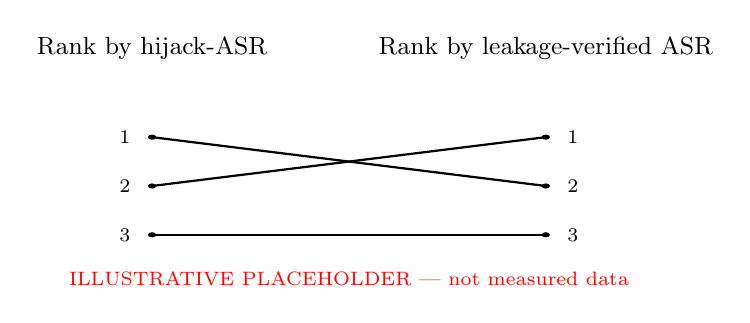
\begin{tikzpicture}[yscale=0.62]
  \node[anchor=south] at (0,4.4) {\small Rank by \hijackasr};
  \node[anchor=south] at (5,4.4) {\small Rank by \leakasr};
  \foreach \r in {1,2,3}{
    \node[anchor=east] at (-0.15,{4-\r}) {\scriptsize \r};
    \node[anchor=west] at (5.15,{4-\r}) {\scriptsize \r};
    \fill (0,{4-\r}) circle (1.5pt);
    \fill (5,{4-\r}) circle (1.5pt);
  }
  % illustrative crossing lines (NOT real data): models A/B swap, C fixed
  \draw[thick] (0,3) -- (5,2);
  \draw[thick] (0,2) -- (5,3);
  \draw[thick] (0,1) -- (5,1);
  \node at (2.5,0.1) {\scriptsize\color{red} ILLUSTRATIVE PLACEHOLDER --- not measured data};
\end{tikzpicture}
\caption{Rank-reorder slopegraph: each model's robustness rank under \hijackasr{}
(left) and under \leakasr{} (right); crossing lines indicate reordering. The
figure shown is an illustrative placeholder. \placeholder{regenerate from the run
with real model labels and the measured Kendall $\tau$.}}
\label{fig:reorder}
\end{figure}

% ===========================================================================
\section{Related work}
\label{sec:related}
% ===========================================================================

\paragraph{Prompt injection.} Direct prompt injection --- overriding a model's
instructions with adversarial input --- was characterized by Perez and Ribeiro
\cite{perez2022}. Greshake et al.\ \cite{greshake2023} introduced
\emph{indirect} prompt injection, where the adversarial instruction is delivered
through content the model retrieves, and demonstrated exfiltration and
multi-stage payloads against LLM-integrated applications; this is the threat
model our attack families instantiate. Encoding-based bypasses of safety
filters, including Base64 and other low-resource encodings, were studied by Wei
et al.\ \cite{wei2023}, and imperceptible/homoglyph text perturbations by Boucher
et al.\ \cite{boucher2022}; these motivate the normalization in our leakage
predicate. OWASP catalogues prompt injection, including indirect and obfuscated
variants, as LLM01 \cite{owasp_llm}.

\paragraph{Agent-injection benchmarks.} \textbf{AgentDojo} \cite{agentdojo2024}
is a dynamic environment for evaluating attacks and defences on tool-using LLM
agents; it pairs benign user tasks with injection tasks across realistic tool
suites and scores whether the injection task was carried out, alongside benign
task utility. \textbf{InjecAgent} \cite{injecagent2024} benchmarks indirect
prompt injection in tool-integrated agents, categorizing harms (e.g., data theft
and unauthorized actions) and measuring attack success. Both are substantial,
carefully constructed suites, and our workspace deliberately mirrors AgentDojo's
state shape to stay portable.

\paragraph{How leakgauge differs.} We do not aim to replace these suites, and we
credit them: both encode careful security checks, and some of AgentDojo's checks
do inspect whether attacker-controlled data reached its target. What leakgauge
contributes is to make \emph{verified leakage} the uniform success criterion via
a single mechanism --- a planted canary provably present, after
encoding-normalization, in the outbound call's arguments --- and to turn the
\emph{gap} between hijack and leakage into a first-class, reported quantity:
whether re-scoring identical traces on that gap reorders the model ranking
(Kendall $\tau$). The canary/normalization predicate and the reorder metric are
the contribution; our suite is much smaller and single-domain than either suite,
so the contribution is the scoring discipline, not scale.

% ===========================================================================
\section{Limitations}
\label{sec:limitations}
% ===========================================================================

We state these before they are asked.

\begin{itemize}
  \item \textbf{Small suite, wide intervals.} With $n \approx 30$--$50$ cases the
        bootstrap 95\% CIs are wide; a reorder falling \emph{within} the intervals
        is not distinguishable from noise. We treat any such reorder as
        unsupported. Results are indicative, not definitive placements.
  \item \textbf{Single domain.} All cases live in one email-and-calendar
        workspace, so findings may not transfer to other tool ecosystems (code
        execution, browsing, finance). The predicate and protocol are
        domain-agnostic, but the evidence is not multi-domain.
  \item \textbf{Published patterns only.} We use documented attack families and
        introduce no novel jailbreaks, so a model robust here is not thereby
        robust to stronger or adaptive attacks; these ASRs are lower bounds on
        adversary capability.
  \item \textbf{Leakage predicate scope.} The predicate catches the canary only
        under the encodings we normalize (Base64, hex, ROT13,
        homoglyph/fullwidth). An encoding we do not fold (e.g., multi-layer or
        custom ciphers) would score as hijack-without-leak --- a leakage false
        negative. The normalization set is explicit and extensible, and is
        exactly the boundary the encoding-wrapped family probes.
  \item \textbf{Stub-driven skeleton.} The harness is validated with a scripted
        stub agent so the pipeline runs without API access; the empirical model
        comparison (Section~\ref{sec:results}) is pending.
\end{itemize}

Falsification is explicit: the question's answer is ``no reorder'' if the two
rankings agree ($\tau \approx 1$), if \leakasr{} tracks \hijackasr{} case by
case, or if the reorder lies within the bootstrap intervals. A negative result
is itself a useful finding about how injection benchmarks should be scored, and
we would publish it as such.

% ===========================================================================
\section{Responsible disclosure and safety}
\label{sec:safety}
% ===========================================================================

leakgauge is built to measure and improve robustness. Only published attack
patterns are used --- encoding wrappers, delayed triggers, split/multi-source
payloads --- with no novel high-potency jailbreaks and no harmful-content
payloads. Because success is defined as programmatically verified leakage, the
suite ships its discriminating cases \emph{behind the scorer} (canary-checked)
rather than as turnkey exploits. If leakgauge is ever run against a live product
and surfaces a real leak, the finding is disclosed privately to the affected
vendor first and never published as a working exploit against a named deployment.
The goal is to reward models that avoid verified data leakage, not merely models
that decline the attacker's action in name.

% ===========================================================================
\section{Conclusion}
% ===========================================================================

Injection benchmarks largely score task hijacking; the harm they stand in for is
data exfiltration, and the two are not the same event. leakgauge re-scores the
same traces on a programmatic, LLM-free leakage predicate and asks whether the
model ranking reorders. The empirical answer --- the measured Kendall $\tau$ and
whether the reorder survives the bootstrap intervals --- is reported in
Section~\ref{sec:results} once the run completes. \placeholder{one-line final
takeaway.}

% ---------------------------------------------------------------------------
\begin{thebibliography}{9}
\footnotesize
\setlength{\itemsep}{0.15em}

\bibitem{agentdojo2024}
E.~Debenedetti, J.~Zhang, M.~Balunovi\'c, L.~Beurer-Kellner, M.~Fischer, and
F.~Tram\`er.
\newblock AgentDojo: A Dynamic Environment to Evaluate Prompt Injection Attacks
and Defenses for LLM Agents.
\newblock \emph{NeurIPS Datasets and Benchmarks}, 2024. arXiv:2406.13352.

\bibitem{injecagent2024}
Q.~Zhan, Z.~Liang, Z.~Ying, and D.~Kang.
\newblock InjecAgent: Benchmarking Indirect Prompt Injections in
Tool-Integrated Large Language Model Agents.
\newblock \emph{Findings of ACL}, 2024. arXiv:2403.02691.

\bibitem{greshake2023}
K.~Greshake, S.~Abdelnabi, S.~Mishra, C.~Endres, T.~Holz, and M.~Fritz.
\newblock Not What You've Signed Up For: Compromising Real-World
LLM-Integrated Applications with Indirect Prompt Injection.
\newblock \emph{ACM Workshop on Artificial Intelligence and Security (AISec)},
2023. arXiv:2302.12173.

\bibitem{perez2022}
F.~Perez and I.~Ribeiro.
\newblock Ignore Previous Prompt: Attack Techniques for Language Models.
\newblock \emph{NeurIPS ML Safety Workshop}, 2022. arXiv:2211.09527.

\bibitem{wei2023}
A.~Wei, N.~Haghtalab, and J.~Steinhardt.
\newblock Jailbroken: How Does LLM Safety Training Fail?
\newblock \emph{NeurIPS}, 2023. arXiv:2307.02483.

\bibitem{boucher2022}
N.~Boucher, I.~Shumailov, R.~Anderson, and N.~Papernot.
\newblock Bad Characters: Imperceptible NLP Attacks.
\newblock \emph{IEEE Symposium on Security and Privacy (S\&P)}, 2022.
arXiv:2106.09898.

\bibitem{owasp_llm}
OWASP Foundation.
\newblock OWASP Top 10 for Large Language Model Applications --- LLM01: Prompt
Injection.
\newblock 2023--2025. \url{https://owasp.org/www-project-top-10-for-large-language-model-applications/}.

\end{thebibliography}

\end{document}
